% Requires:
% \usepackage{pgfplots}
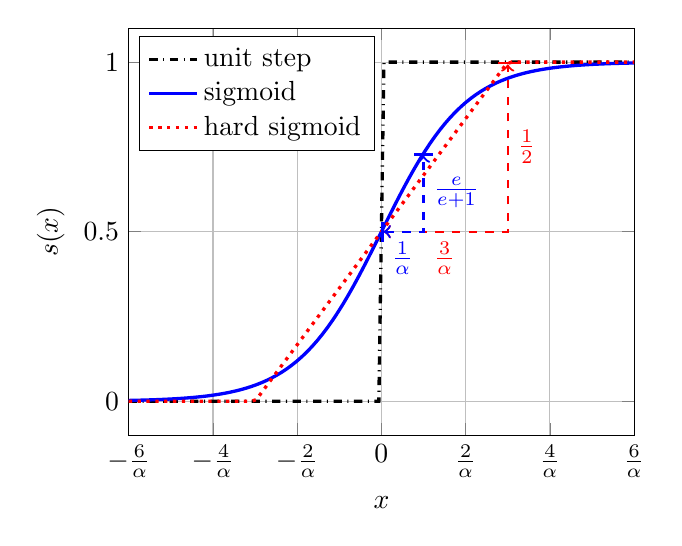
\begin{tikzpicture}[
    declare function={
      sigmoid(\x,\alpha)=1/(1+exp(-\x*\alpha));
      relu6(\x)=min(max(0,\x),6);
      hard_sigmoid(\x,\alpha)=relu6(\x*\alpha + 3)/6;
    }
  ]
  \begin{axis}%
    [
      width=8cm,
      %axis on top,
      grid=major,
      xmin=-6,
      xmax=6,
      %axis x line=middle,
      ytick={0,.5,1},
      ymin=-.1,
      ymax=1.1,
      %axis y line=middle,
      samples=100,
      domain=-6:6,
      xlabel={\(x\)},
      ylabel={\(s(x)\)},
      height=6.75cm,
      xtick={-6,-4,-2,0,2,4,6},
      xticklabels={\(-\frac{6}{\alpha}\),\(-\frac{4}{\alpha}\),\(-\frac{2}{\alpha}\),0,\(\frac{2}{\alpha}\),\(\frac{4}{\alpha}\),\(\frac{6}{\alpha}\)},
      legend style={at={(0.02,0.98)},anchor=north west},
      legend cell align=left,
    ]
    \addplot[black,dash dot,very thick,mark=none]   (x,{x>0});
    \addplot[blue,very thick,mark=none]   (x,{sigmoid(x,1.0)});
    \addplot[red,very thick,dotted,mark=none]   (x,{hard_sigmoid(x,1.0)});
    \legend{unit step,sigmoid,hard sigmoid}

    \draw[|<->|,thick,dashed,red] (axis cs:0.0,0.5) -- (axis cs:3.0,0.5) node[below,midway] {\(\frac{3}{\alpha}\)} -- (axis cs:3.0,1.0) node[right,midway] {\(\frac{1}{2}\)};

    \draw[|<->|,thick,blue,dashed] (axis cs:0.0,0.5) -- (axis cs:1.0,0.5) node[below,midway] {\(\frac{1}{\alpha}\)} -- (axis cs:1.0,0.731) node[right,midway] {\(\frac{e}{e+1}\)};
  \end{axis}
\end{tikzpicture}
